\begin{center}
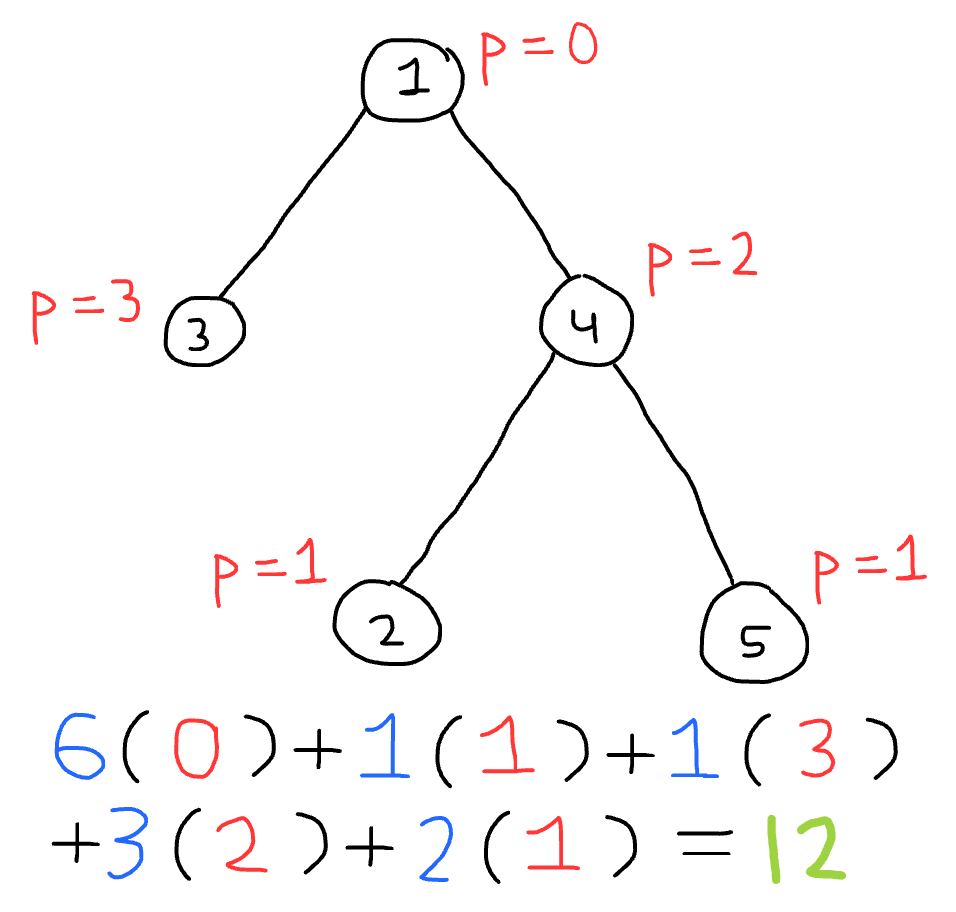
\includegraphics[scale=0.5]{Drawing-5.sketchpad.png}
\end{center}

The diagram above illustrates the first test case. An optimal set of operations to perform is to upgrade tower $3$ a total of $3$ times, upgrade tower $4$ twice, and upgrade towers $2$ and $5$ once each. This gives us a total cost of $12$, which is the minimum possible. Note that there may be other valid sets of operations with the same minimum cost.
